\documentclass[10pt, twocolumn]{article}
\usepackage[margin=1in]{geometry}
\usepackage{graphicx}
\usepackage{subcaption}

\title{Deep Reinforcement Learning for Atari Games}
\author{Garnet Liu \and Vikram Saraph \and Birol Senturk}

\begin{document}
\maketitle

\begin{abstract}

Abstract here.

\end{abstract}

\section{Introduction}

In recent years, deep learning techniques have been successfully adapted and applied to problems
in reinforcement learning. In this project, we survey and evaluate one such technique, called \emph{imagination augmented agents},
(or \emph{I2A}). This technique was initially developed and published by Weber \emph{et. al.} at DeepMind \cite{}. In their original
work, the authors describe the novel I2A as one that combines aspects of \emph{model-free} learning, in which an agent makes decisions
based only on its current observations, with \emph{model-based} learning, where the agent attempts to learn about its environment
in addition to a policy. In their work, the model-free agent is augmented with a model-based \emph{imagination engine}, which
makes predictions about future trajectories of the agent from its current state.

While model-free agents have seemingly more flexible architectures, in practice they do not generalize do different tasks. Incorporating 
model-based aspects allows one to provide additional fine-tuning to the network's architecture in some way that is representative of the 
agent's environment. Indeed, the authors of the original paper demonstrate a significant improvement in the agent when adding 
imagination to a standard model-free agent. They evaluate I2A on two different 2d games: MiniPacman, which is a simplified version of 
PacMan, and Sokoban, in which the agent must push blocks onto designated targets.

In this work, we focus on applying I2A to Pong. We 

\section{Related Work}
Previous work on model-free agents, and model-based agents. Borrow content from the related work section in the original paper.

\section{Background}

In this section, we provide a high-level overview of the I2A architecture as described in the original work. See the Methodology section for more specifics on how we applied this architecture to our Pong use case.

I2A unifies a model-free 
architecture and a model-based one. The model-based component of I2A is also referred to as the imagination engine, and consists of a 
sequence of \emph{imagination cores} that collectively generate a predicted future trajectory. Each imagination core makes use of a pre-trained policy network and an environment model. The policy network simply predicts the best action to take given an input state. The environment model takes an input state and the action returned by the policy network, and predicts the next state from taking the action. The predicted next state is fed from one imagination core to the subsequent one, so in this way, the output of the imagination cores is a sequence of predicted states (or trajectory). This trajectory provides additional context when learning a policy; together, the model-free policy and the imagine engine are combined to train a unified policy.

\section{Dataset}
We use the Arcade Learning Environment (ALE) to simulate playing Atari games. ALE has been integrated
into OpenAI Gym, which provides a standardized interface for taking actions and retrieving the resulting new
state, reward, etc. The game's state is simply the RGB image of a frame at a given point in time.

Before image data is fed into any part of the network, it is normalized in a way that is more convenient for training.
In particular, the top the image is removed, since it is only used to display the players' scores, pixels of which are
unlikely to be useful features. In addition, the top and bottom border color is changed from white to black, since
it is the same color as the ball. The idea is to help the network distinguish between the two types of pixels.
See Figure \ref{screenshots} below.

\begin{figure}[h]
\centering
\begin{subfigure}[b]{.2\textwidth}
  \centering
  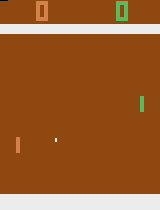
\includegraphics[scale=0.5]{unnormalized}
  \caption{Original image}
  \label{fig:unnormalized}
\end{subfigure} 
\begin{subfigure}[b]{.2\textwidth}
  \centering
  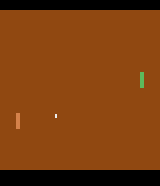
\includegraphics[scale=0.5]{normalized}
  \caption{After normalization}
  \label{fig:normalized}
\end{subfigure} \hfill
\caption{Pong screenshots before and after normalization}
\label{screenshots}
\end{figure}

The OpenAI Gym API provides rewards and states, so we work with this data when training our model.
Actions are taken with the \verb|step| function, which returns the resulting data.

\section{Methodology}

The model is trained in three phases. First, a model-free agent is trained by playing the game and using
A2C to learn. Once the model-free agent is trained, its policy is used to train the environment model.
The environment is trained by using the model-free agent's policy to play the game; by doing so it learns the
environment. In the following, we outline the structure of our TensorFlow program.

\begin{figure*}
\centering
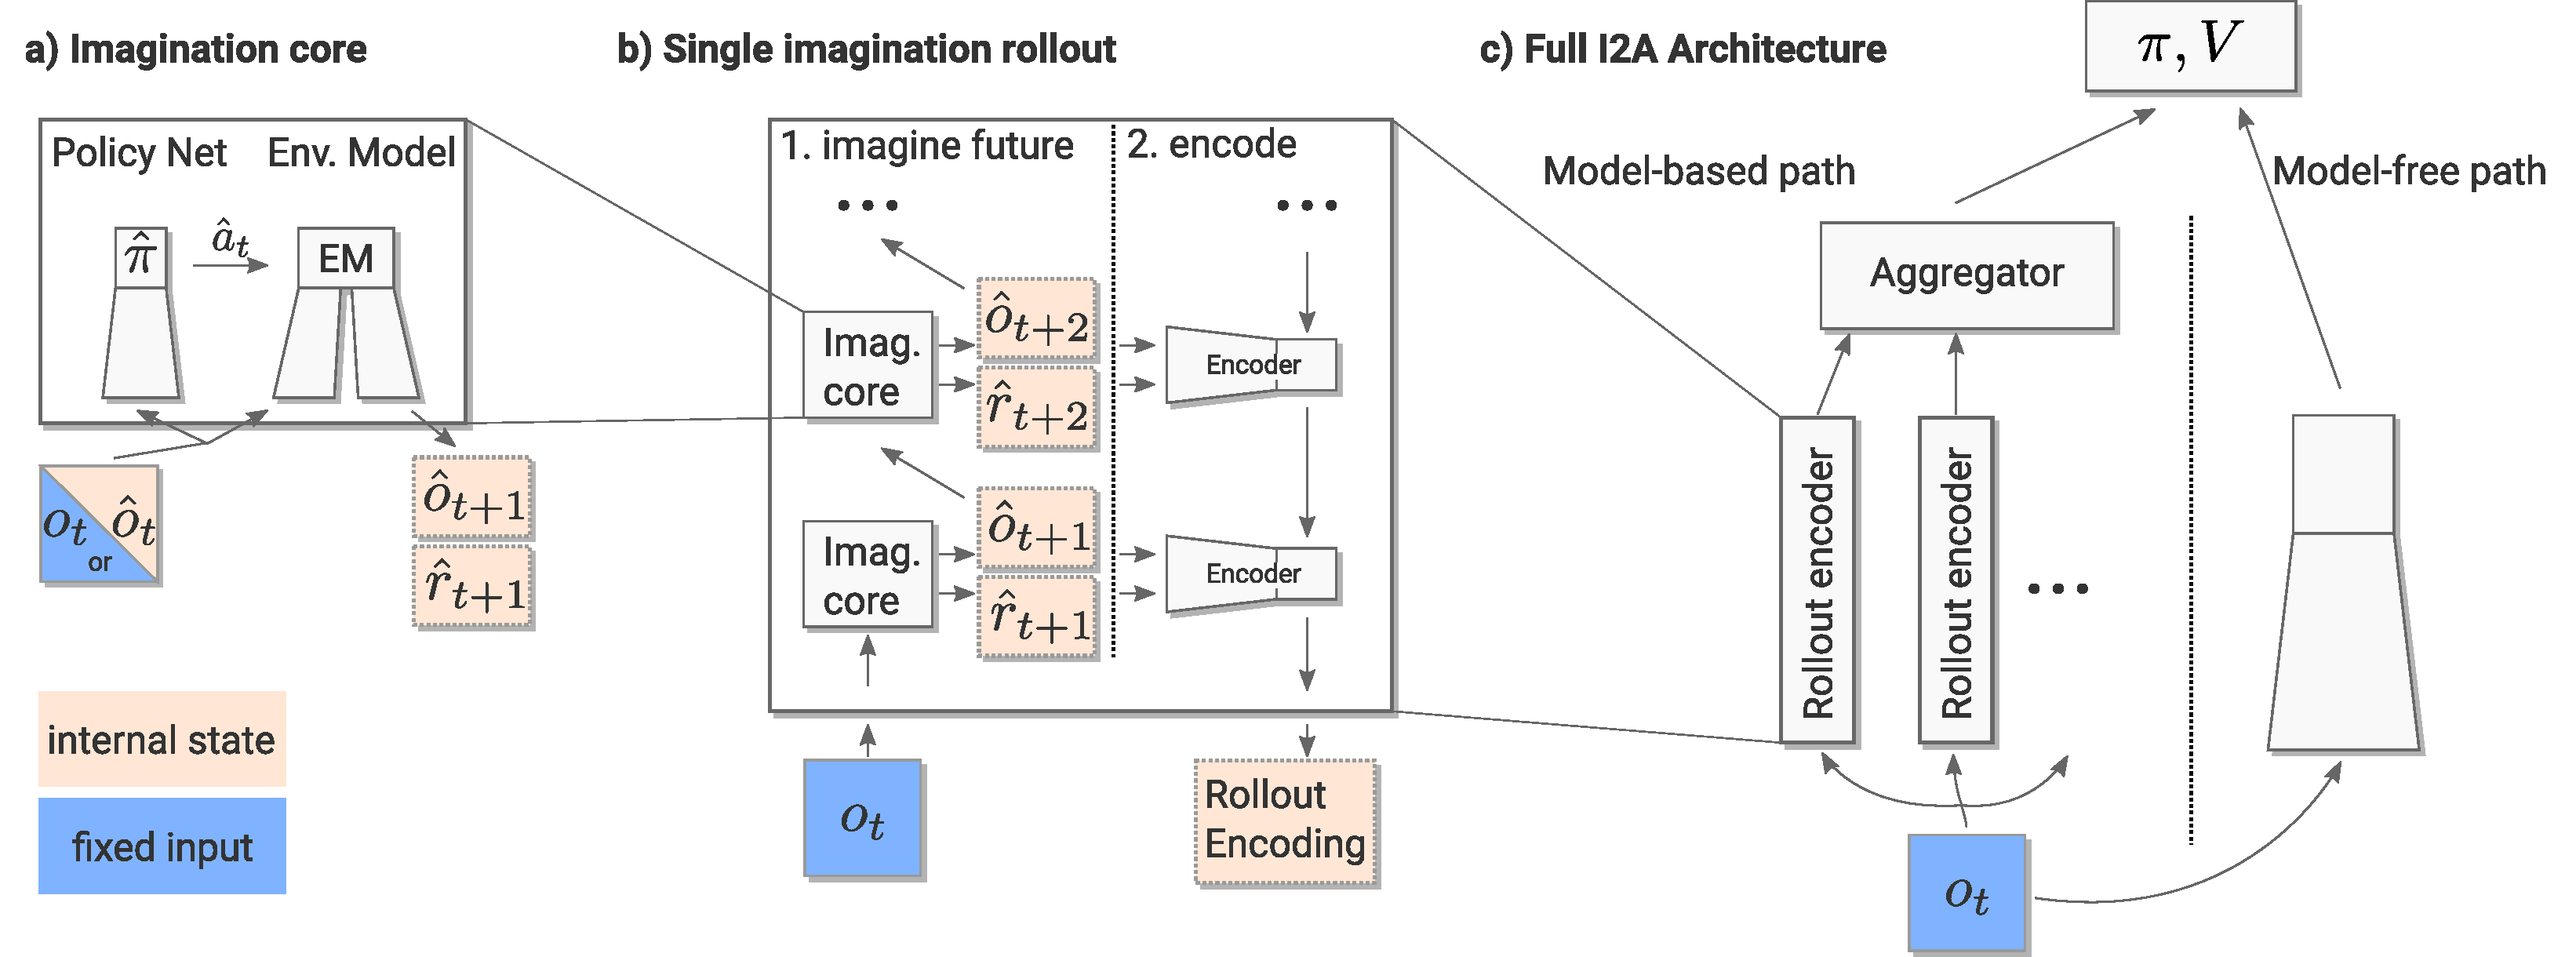
\includegraphics[scale=0.3]{i2a}
\caption{I2A architecture}
\end{figure*}

\subsection{Model-free agent}

\subsection{Environment model}

The computation graph of the environment model's network begins by using the policy described in the
previous section to take an action. Given an action and current state, recall that the environment model
predicts the next state and reward obtained. In general, the environment model's architecture should be
designed for the specific game in mind; however, for this project we used a modified version of the
MiniPacman environment model.

Recall that the state returned by the OpenAI Gym API is just an RGB image, and due to normalization 
described in the Dataset section, there are only five distinct kinds of pixels: border pixels (black),
background pixels (brown), ball pixels (white), player pixels (green), and opponent pixels (orange).
Therefore, the each pixel in a given state is first mapped to a corresponding index (1 - 5). Then, the action
taken by the model-free agent is converted to a one-hot representation, and concatenated to the
state data. This encodes all state and action information that the environment model needs to begin training.

Next, the input data is sent through a series of convolutional layers, consisting of higher level logical units
called ``basic blocks", as described in the paper. The first layer of a basic block is \emph{pool-and-inject},
which applies a maxpool and concatenates the result to the input. The result is then passed though
convolutional layers, the output of which is the final output of a basic block.



\subsection{I2A}

I2A combines the knowledge learned by the models from the previous two steps.

\section{Results}

\subsection{Imagination}

\section{Discussion}

\subsection{Limitations}

\end{document}